\chapter*{Proposition 39}



\begin{figure*}[ht]
    \begin{center}
    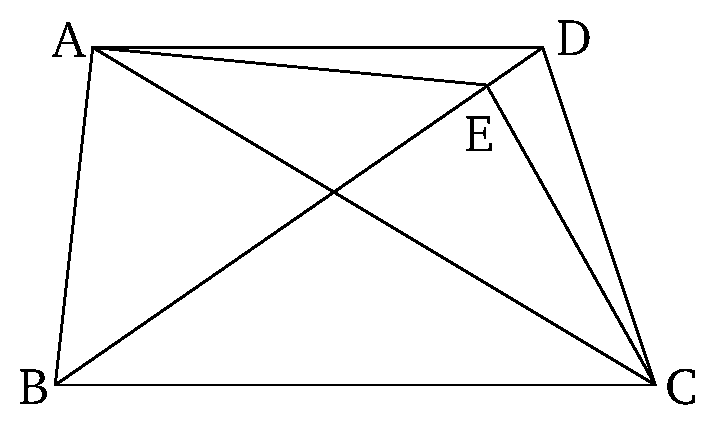
\includegraphics[width=0.5\linewidth]{figures/fig39e.eps}
    \label{fig:prop_39}
    \end{center}
\end{figure*}

Equal triangles which are on the same base, and on the same side, are
also between the same parallels.

Let $ABC$ and $DBC$ be equal triangles which are on the same base $BC$,
and on the same side (of it). I say that they are also between the same parallels.

For let $AD$ have been joined. I say that $AD$ and $BC$ are parallel.

For, if not, let $AE$ have been drawn through point A parallel to the straight-line $BC$ [Prop.~1.31], and let $EC$ have been joined. Thus, triangle $ABC$ is equal
to triangle $EBC$. For it is on the same base as it, $BC$, and between the
same parallels [Prop.~1.37]. But $ABC$ is equal to $DBC$. Thus, $DBC$ is
also equal to $EBC$, the greater to the lesser. The very thing is impossible.
Thus, $AE$ is not parallel to $BC$. Similarly, we can show that neither (is)
any other (straight-line) than $AD$. Thus, $AD$ is parallel to $BC$.

Thus, equal triangles which are on the same base, and on the same side, are
also between the same parallels. (Which is) the very thing it was required to show.


\section*{Commentary}

\begin{proposition}\label{proposition_39}\lean{Elements.Book1.proposition_39}\leanok
    If
\end{proposition}
\begin{proof}
    \uses{proposition_31,proposition_37}\leanok
\end{proof}
